
\section{Resultados}

\subsection{Obtencion de datos en formato String}
Se utilizan los tres metodos mencionados en la seccion de Materiales y Metodos.

\subsubsection{bitR}
Para este analisis hemos usado el paquete bitR de Rstudio. Hemos realizado un bitR del proteoma humano para un score maayor de 650. Posteriormente hemos comprobado cuantas de las proteinas humanas de nuestra tabla de union con covid se encuentra en nuestro proteoma obtenido. Posteriormente, hemos comprobado cuantas de ellas estan unidas a genes covid, y cuantos genes covid son.

\subsubsection{biomaRt}
Para este analisis hemos utilizado un paquete de Rstudio llamado biomaRt. Este paquete nos permite cambiar la codificacion de uniprot a ensamble.
El codigo perteneciente a este analisis se encuentra en la carpeta code y se denomina biomart.R. En este codigo viene detallado con comentarios el
proceso que se ha llevado a cabo. Basicamente los pasos seguidos son: 
- pasar de codigo uniprot a ensamble
- comprobar cuantos de estos codigos ensamble se encuentran en el proteoma completo, guardamos en un dataframe los valores ensamble y uniprot.  Comprobamos que solo nos quedamos de 332 proteinas humanas unidas a viricas con 107.
- Hacemos un bucle y guardamos en un dataframe los valores de uniprot y ensamble aquellos que coinciden con nuestra tabla de entrada.
- Hacemos un merge que nos une los dos dataframe, el de entrada con genes covid y humanos, y el obtenido con el cambio de uniprot a ensamble. 


\subsubsection{Tabla UniProt}
Para este analisis hemos utilizado una tabla obtenida de la base de datos de UniProt, que contiene tres columnas. Un valor de uniprot, uno de ensamble y otro tipo de codigo uniprot para el mismo gen. 
El codigo perteneciente a este analisis se encuentra en la carpeta code y se denomina tablaObtenidaUniprot.R. Nuevamente en el codigo vienen detallados los pasos seguidos. 
El proceso llevado a cabo es el siguiente:
- Leemos los ficheros: la tabla de uniprot, la tabla de relaciones entre genes viricos y humanos, y el proteoma de interaccion completo. El fichero con la tabla de uniprot tiene filas que no contienen codigo ensamble para algunos de los genes. Asi que realizaremos un filtrado que elimine estas filas.
- Una vez realizado esto, buscaremos cuantos de estos codigos ensamble se encuentran en el proteoma completo. Vemos que solo perdemos cuatro de estos codigos.
- Posteriormente, buscaremos cuantos de los codigos uniprot de mi tabla de entrada podemos convertir a ensamble. 


\subsection{Obtencion del grafo de relaciones proteinascovid-proteinasHumanas}

Para abordar el problema de la creacion de un grafo conexo, nos hemos enfrentado a tiempos de ejecucion elevados y un gasto de memoria elevada. 
El codigo denominado AlgoritmoRedCompleta.R muestra como se ha llevado a cabo el proceso de obtencion de red. 
Una vez obtenido en el apartado anterior la tabla con nuestros genes uniprot en formato string, ya podriamos usar funciones pertenecientes a igraph que buscaran rutas entre una y otra proteina humana dentro del proteoma. 
Como primer paso se intento obtener todas las rutas posibles entre todas las proteinas humanas unidas al covid, usando la función all simple paths. 
Nos enfrentamos a una compilacion donde tras 15 horas de ejecucion continua nuestro código no había terminado de definir las rutas entre las proteinas,además de haber generado un archivo de casi 15 gigas que por poco ocupaba toda la memoria de R. 
Decidimos hacer una pequeña modificaciones y calcular todas las rutas posibles con la misma funcion pero simplemente haciendo las combinaciones de un gen con su siguiente. Nuevamente el tiempo de ejecucion y la memoria ocupada eran inviables. 
Tambien se investigo el parametro cuttof que permitia establecer un tamaño minimo del camino, pero tampoco conseguiamos un resultado que su tiempo de ejecucion fuera factible. 
Asi que, tras varios dias de prueba, decidimos usar la función all shortest path, que obtenia la ruta mas rapida de una proteina a otra. Creíamos que esto seria más rapido y obtendriamos los resultados necesarios para poder obtener el grafo. Pero nuevamente, vimos que el tiempo y la memoria que se ocupaba eran enormes. Otra opcion era comparar una proteina con su siguiente, pero esto tras 5 horas y 8 gigas no habia terminado de compilar. 
Como ultima opción, decidimos hacer una simplificacion. Cogimos 2 genes humanos por cada gen de covid, e hicimos un dataframe. Este dataframe es el que usamos para obtener el grafo completo. 
Probamos dos opciones, una de ellas utilizaba todas las combinaciones posibles entre estas dos proteinas de cada gen (51 proteinas en total) y la otra utilizaba una proteina con su siguiente. Para optimizacion de tiempo y memoria usamos la segunda de las opciones, obteniendo 100 elementos donde cada una tenia varias listas de uniones de grafos. Como muchas de ellas se repetian usamos unique y conseguimos reducir estas repeticiones. Obteniendo 18012 rutas, que seguiamn teniendo elementos repetidos. A continuación, creamos dos vectores, y hacemos un bucle que vaya recorriendo estas rutas, y me vaya añadiente una proteina en un vector, y la proteina con la que interacciona en el siguiente. Todo esto se integra en un data frame y usamos unique para eliminar las repeticiones. 
Este dataframe lo convertimos en objeto igraph y mediante el operados de unión conseguimos unir dos objetos igraph, esto unira los dos objetos igraph y ya podremos comprobar si hemos obtenido o no la componete conexa usando la función components. Es importante mencionar que para poder crear las rutas, nuestro grafo de proteoma debe tener una unica componente conexa, y si tiene mas de una, las proteinas buscadas pertenezcan al mismo. El resultado se comentara en el apartado de discusiones. 

\begin{figure}[ht!]
	\centering
	\includegraphics[scale = 0.3]{figures/allSimplePathUnaProt.png}
	\caption{Captura del tamaño de rutas creadas,sin compilacion completa con función all simple paths}
\end{figure}

\begin{figure}[ht!]
	\centering
	\includegraphics[scale = 0.3]{figures/allShortestPathsTODOS.png}
	\caption{Captura del tamaño de rutas creadas,sin compilacion completa con función all shortest paths}
\end{figure}



\subsection{Analisis de propiedades del grafo obtenido}
Realizaremos un analisis exahustivo de la red obtenida, analizando las propiedades estudiadas en clase.

\subsubsection{Comparacion entre la red obtenida y la red humana}
Encontramos los resultados de esta parte en la carpeta code y el codigo AnalisisRedFinal.R. Se estudian las siguientes componentes:
- Densidad: es considerada como una medida de cohesion entre los nodos de la red. Es una medida del numero de vinculos existentes en la red, presentados como una proporcion del numero de vinculos posibles. 
  * Densidad red proteoma humano: 0.03
  * Densidad red obtenida: 0.002
- Reprocidad: es una medida de probabilidad de que los vértices de una red dirigida se vinculen mutuamente entre sí. En general las redes reales tienen una reprocidad entre 0 y 1. Obtenemos un 1 para ambas redes.
- Diametro: se denomina asi al máximo camino más corto entre dos nodos medido por el numero de elnaces recorrido. Un diametro menor indica mayor habilidad de comunicacion en la red. Debe preocurarse que el diametro de las redes de intercomunicación sea lo más pequeño posible. 
  * Diametro red proteoma humano: 5
  * Diametro red obtenida: 7
  
  \begin{figure}[ht!]
	\centering
	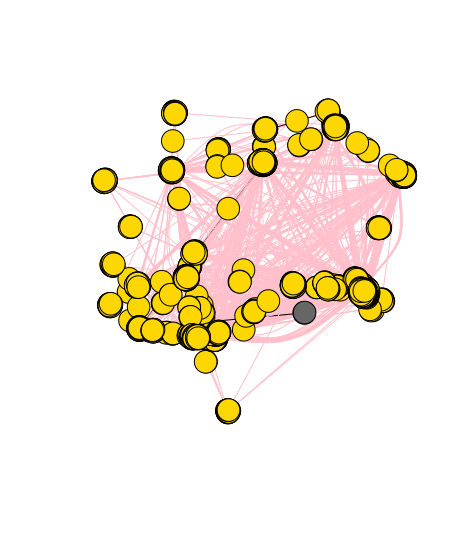
\includegraphics[scale = 0.3]{Rplot01.png}
	\caption{Representacion del diametro de la red conseguida}
\end{figure}

- Grado: es el número de conexiones de un vertice o nodo con otros nodos. 
  * Grado maximo red proteoma humano: 15014, solo para un nodo
  * Grado minimo red proteoma humano: 2, para 16 nodos
  * Grado maximo red obtenida: 620, solo para un nodo
  * Grado minimo red obtenida 1, parao 208 nodos
- Distribución de grado: la distribución de grado en una red representa habitualmente como P(K) y es definida como la fraccion de nodos en la red con un cierto grado k. 
- Distancia media: es el promedio o media de las distancias entre vertices en un grafo conexo, es una medida natural de la compacidad del grafo. 
  *Distancia media red proteoma humano: 2.040557
  *Distancia red obtenida: 3.517751
- Asortatividad: es la preferencia de los nodos de una red por unirse a otros que le son similares en alguna caracteristicas. Habitualmente se estudia en funcion del grado.
  *Asortatividad red proteoma humano: 0.1040102
  *Asortatividad red obtenida:-0.55738

\subsubsection{Modularidad}

Para obtener la modularidad del grafo hemos usado el paquete igraph. El codigo correspondiente se encuentra en un archivo llamado Modularidad y Centralidad.R
Lo primero fue obtener los modulos del grafo mediante la función cluster walktrap. Obtuvimos 68 grupos de tamaño diverso, desde 4 hasta 1778. Una vez obtenido esto, se le pasa a la funcion modularity transformándolo a un vector de membership (con la funcion membership) y pasando el grafo original como parámetro. El resultado es una modularidad de 0.935.
Despues de esto, representamos algunos valores pertinentes, como una lista de los tamaños de los grupos y Grafo en el que solo se ven los modulos coloreados.
Este grafo se hizo con plot.igraph, y nos muestra los 68 modulos por separado.
Aparte, vimos la posibilidad de representar un dendograma, pero no aporta ninguna informacion util debido a la cantidad de datos.


\subsubsection{Centralidad}

Tras realizar el an\'alisis de componentes, se ha observado que el m\'etodo de centralidad ganador ha sido el de \textbf{cercan\'ia}(closeness) de \textit{Spearman}. Dicho método considera como importancia aquellos nodos que están más cercanos de media al resto de nodos.
Una vez escogido el m\'etodo de closeness, se ha realizado el estudio de la centralidad con la funci\'on \textit{closeness} del paquete \textbf{igraph}. Dicha funci\'on nos ha otorgado la centralidad de cada nodo respecto al sistema de manera normalizada(Valores de entre cero y uno).
Analizando estos resultados, se ha obtenido que la media de la centralidad de los nodos de la red es \textbf{0.287}.
Adem\'as se ha calculado cuantos nodos de la red usada(subgrafo de la red que forma una sola componente conexa) tienen ciertos valores de centralidad.
En primer lugar, ho hay ningún valor de centralidad menor que 0.1. Con un valor de centralidad entre 0.1 y 0.3 hay un total de 1990 nodos, mientras que hay 898 nodos que presentan un valor de modularidad de entre 0.3 y 0.5. Por último, no hay ningún nodo con un valor de centralidad mayor de 0.5.


\subsubsection{Robustez}

Para comprobar la robustez de nuestro grafo vamos a realizar dos ataques dirigidos, uno basado en degree y otro en betweenness. En ambos casos representaremos el numero restante de nodos conexos por cada ataque en una grafica. Tras obtener los resultados, podemos observar que el ataque basado en betweenness deshace el grafo mucho mas rapido que el de degree. Esto tiene sentido ya que eliminar nodos clave con muchas uniones es muy eficaz. De hecho podemos ver que con el primer ataque ya reducimos la red de 9000 nodos a poco mas de 3000. Por tanto podemos deducir que hay un solo nodo que unia varios grupos de gran tamaño.
El ataque por degree es mucho mas gradual, pero aun asi deshace el grafo en aproximadamente 35 ataques.

\subsection{Enriquecimiento funcional}

El enriquecimiento funcional realizado est\'a en dos tablas distintas, una para cada columna de la tabla de genes que forma nuestro subgrafo.\newline
\begin{figure}[ht!]
	\centering
	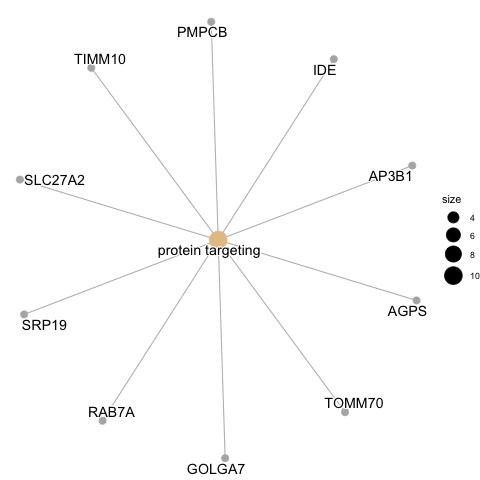
\includegraphics[scale = 0.2]{figures/GenesProteinTargeting.png}
	\caption{Genes que participan en \textit{Protein Targeting, GO:0006605}}
\end{figure}
De las dos tablas obtenidas observamos que la primera solo contiene una fila de un t\'ermino GO que es un proceso biol\'ogico. Dicho t\'ermino es \textbf{GO:0006605} y es un proceso biol\'ogico que hace referencia a orientar a prote\'inas espec\'ificas a regiones particulares de una c\'elula, normalmente a \'organulos celulares delimitados por membrana.
En la segunda tabla tenemos una gran multitud de t\'erminos de \textit{GO} apuntados. En total hay 2120 t\'erminos de los cuales 1586 son \textit{procesos bi\'ologicos}, otros 237 son \textit{funciones moleculares} y los \'ultimos 297 son \textit{componentes celulares}.\newline
En este caso como nos encontramos con una gran cantidad de t\'erminos no los nombraremos uno por uno sino que se mostrar\'an los t\'erminos que se consideren m\'as importantes mediante un diagrama de barras como con una red con las principales funciones. \newline
\begin{figure}[ht!]
	\centering
	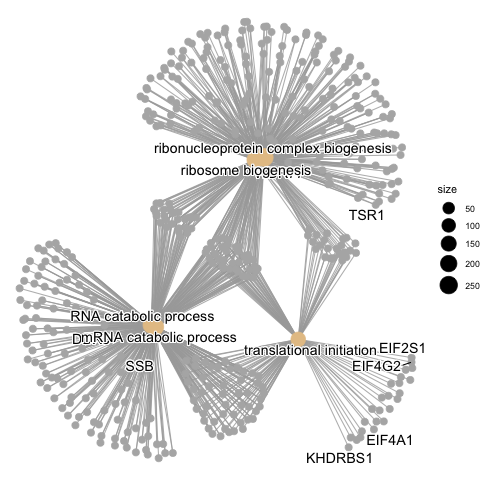
\includegraphics[scale = 0.2]{figures/Genes2Funciones.png}
	\caption{Red de funciones principales del segundo vector de genes}
\end{figure}

\begin{figure}[ht!]
	\centering
	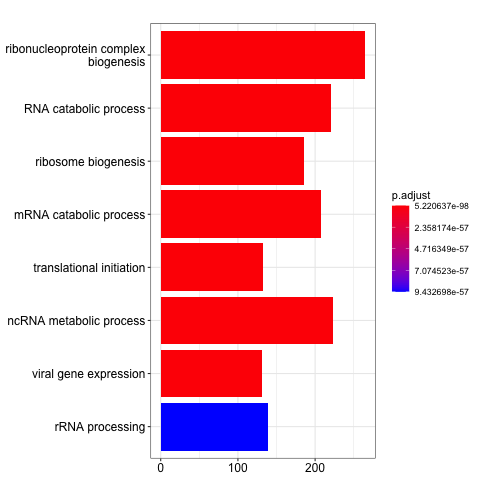
\includegraphics[scale = 0.3]{figures/barplotGenes2.png}
	\caption{Diagrama de las funciones m\'as importantes}
\end{figure}
\clearpage

